\newcommand{\TITLE}{User Manual}
\newcommand{\VERSION}{0.0}

\documentclass[a4paper, oneside, 11pt]{report}
    \usepackage[T1]{fontenc}
    \usepackage[utf8]{inputenc}
    \usepackage[nswissgerman, english]{babel}
    \usepackage[hyphens]{url}
    \usepackage[hidelinks]{hyperref}
    \usepackage{graphicx}
    \usepackage{subfig}
    \usepackage{vhistory}
    \usepackage{float}
    \usepackage{pdfpages}
    \usepackage{tcolorbox}
    \usepackage{xcolor}
    \usepackage{nameref}
    
    % Seitenränder
    \usepackage{geometry}
    \geometry{
        a4paper,
        left=20mm,
        top=30mm,
        right=20mm,
        bottom=30mm
    }

    % Jede Überschrift 1 auf neuer Seite
    \let\stdsection\section
    \renewcommand\section{\clearpage\stdsection}

    % Header and footer
    \usepackage{fancyhdr}
    \pagestyle{fancy}
    \fancyhf{}
    \lhead{\small \TITLE \\ \vspace{0.5mm} \normalsize \nouppercase\leftmark \vspace{0.0cm}}
    \rhead{
        \begin{picture}
            (0,0) \put(-100,0){
\includegraphics[width=0.2\linewidth]{./assets/logo/hsr.png}}
        \end{picture}}
    \cfoot{\thepage}

    % Multicolomns
    \usepackage{multicol}
    \setlength{\multicolsep}{2.0pt plus 2.0pt minus 1.5pt}% 50% of original values (above/below multicols)

    % Chapter ohne Nummerierung, Eintrag in Inhaltsverzeichnis
    \newcommand{\kapitel}[1]{
        \stepcounter{chapter}\chapter*{#1}
        \addcontentsline{toc}{chapter}{#1}
        \markboth{\arabic{chapter} #1}{\arabic{chapter} #1}
    }
    % Section ohne Nummerierung, Eintrag in Inhaltsverzeichnis
    \newcommand{\sectionroman}[1]{
        \stepcounter{section}\section*{#1}
        \addcontentsline{toc}{section}{#1}
        \markboth{\arabic{section} #1}{\arabic{section} #1}
    }

    % Anpassung der Inhaltsverzeichnis-Tiefe, beginnend bei section
    \renewcommand{\partname}{}
    \renewcommand{\thesection}{\arabic{section}}
    \setcounter{secnumdepth}{3}
    \setcounter{tocdepth}{3}

    % Code Listings
    \usepackage{listings}
    \usepackage{color}
    \usepackage{beramono}

    \definecolor{bluekeywords}{rgb}{0,0,1}
    \definecolor{greencomments}{rgb}{0,0.5,0}
    \definecolor{redstrings}{rgb}{0.64,0.08,0.08}
    \definecolor{xmlcomments}{rgb}{0.5,0.5,0.5}
    \definecolor{types}{rgb}{0.17,0.57,0.68}

    \lstdefinestyle{visual-studio-style}{
        language=[Sharp]C,
        columns=flexible,
        showstringspaces=false,
        basicstyle=\footnotesize\ttfamily, 
        commentstyle=\color{greencomments},
        morekeywords={partial, var, value, get, set},
        keywordstyle=\bfseries\color{bluekeywords},
        stringstyle=\color{redstrings},
        breaklines=true,
        breakatwhitespace=true,
        tabsize=4,
        numbers=left,
        numberstyle=\tiny\color{black},
        frame=lines,
        showspaces=false,
        showtabs=false,
        escapeinside={£}{£},
    }
    \lstset{style=visual-studio-style}


\begin{document}

    \begin{titlepage}
	\centering
	\begin{figure}
		\centering
		
\includegraphics[width=0.7\linewidth]{./assets/logo/hsr.png}  	
	\end{figure}
	\
	\vfill
	{\huge\bfseries \TITLE\par}
	\vspace{5mm}
	{\scshape\Large Study Thesis\par}
	\vspace{2mm}
	{\scshape\small Fall Term 2018}
	\vfill

	{\Large\textbf{Authors:} \\\vspace{0.2cm}}
	{\Large Claudio \textsc{Mattes} \\\small claudio.mattes@hsr.ch \par\vspace{0.2cm}
	\Large Lukas \textsc{Kellenberger} \\\small lukas.kellenberger@hsr.ch}

	\vspace{0.6cm}
	{\Large\textbf{Supervisor:} \\\vspace{0.2cm}}
	Cyrill \textsc{Brunschwiler}  \\ {\small Hochschule für Technik Rapperswil} \\\small cyrill.brunschwiler@hsr.ch \\

	% \vspace{0.6cm}
	% {\Large\textbf{Co-Examiner:} \\\vspace{0.2cm}}
	% Title Firstname \textsc{Lastname}  \\ {\small Hochschule für Technik Rapperswil} \\\small Firstname.lastname@hsr.ch \\

	\vfill
	{\scshape\scriptsize Departement Computer Sciences \\ HSR University of Applied Sciences Rapperswil \\ CH-8640 Rapperswil, Switzerland \par}
	\vfill

    % Bottom of the page
    {\large \today}
\end{titlepage}
    \tableofcontents
    \addcontentsline{toc}{part}{Table of Contents}
    \setcounter{section}{1}
    
\kapitel{General Information} \label{GeneralInfo}
\thispagestyle{plain}
\renewcommand\section{\stdsection}
\setcounter{section}{1}
\subsection{System Overview}
The ''System Readiness Inspector'' is a PowerShell tool that helps you to check the readiness of a system to detect advanced persistent threats and lateral movement.After the SRI ran successfully it generates a PDF-Document showing wrong or missung configurations. The SRI was developed during a student research project by the two bachelor of science in computer science students, Claudio Mattes and Lukas Kellenberger.
\\\\
The SRI has four different modes: Online, Offline, GroupPolicy, AllGroupPolicies. The online mode is limited to the current system and thus determines readiness. The offline mode is used to be able to make a statement about any system by means of exports.
The GroupPolicy mode is limited to a specific Group Policy, which is checked for its
audit settings. In the AllGroupPolicies mode, all group policies of the current domain are examined.

\subsection{Organization of the Manual}
The user manual consists of five parts: 
\begin{itemize}
    \item \textbf{General Information:} \ \\
The General Information section explains the tool and the purpose for which it is intended.
    \item \textbf{System Requirements: } \ \\
The System Requirements section provides a general overview of the system requirements. Which operating systems are supported, what software must be pre-installed, and what authorizations the user must have.
    \item \textbf{Getting Started: } \ \\
The Getting Started section explains how to obtain and install the SRI on your device. 
    \item \textbf{Using SRI: }\ \\
The Use SRI section provides a detailed description of the system functions. 
\end{itemize}

    
\kapitel{System Summary}
\thispagestyle{plain}
\renewcommand\section{\stdsection}
\setcounter{section}{2}
\subsection{Operating System}
The SRI runs on all Windows 10 Pro operated systems as well as on all servers with the operating system Windows Server 2016.
\subsection{User Authorizations}
To run the SRI successfully the user needs administrator rights.
\subsection{Pre-Installed Software}
To enable the SRI to read the Resultant Set of Policies, the Remote Server Administration Tools must be installed on the device.
\\\\
This Microsoft tool can be downloaded here: \ \\
\url{https://www.microsoft.com/en-us/download/details.aspx?id=45520}
\\\\
It's easy to install with just a few clicks.
    
\kapitel{Getting Started}
\thispagestyle{plain}
\renewcommand\section{\stdsection}
\setcounter{section}{3}
\subsection{Download}
You can find the latest version of the SRI in this GitHub repository: \\\\
\url{https://github.com/clma91/studythesis/}
\\\\
You download a ZIP folder, which has to be unpacked first.
\subsection{Installation}
You have either downloaded SRI from the official GitHub repository or received it from another source. No further installation is required. The SRI is ready to use.
    
\kapitel{Using SRI}
\thispagestyle{plain}
\renewcommand\section{\stdsection}
\setcounter{section}{4}
\subsection{Starting SRI}
Open Windows PowerShell as administrator:

\begin{figure}[H]
    \centering
    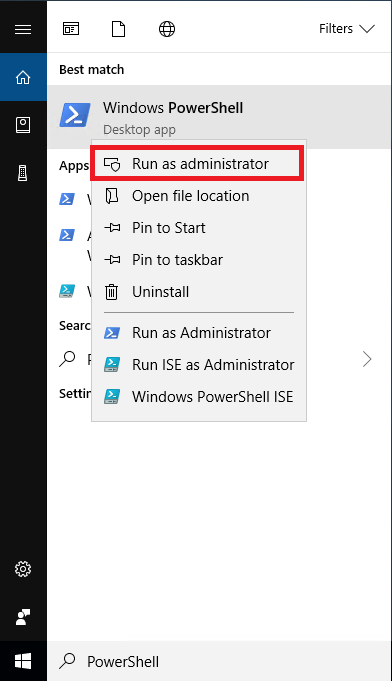
\includegraphics[width=0.35\linewidth]{assets/ps_admin.png}
    \caption{Open PowerShell as Administrator}
\end{figure} \ \\
Navigate to the path the SRI is saved:
\begin{figure}[H]
    \centering
    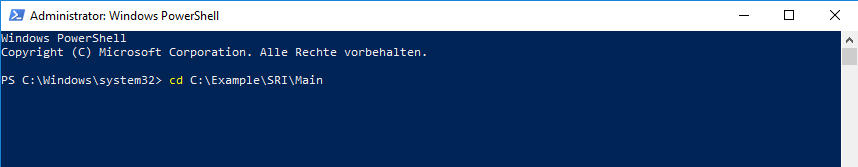
\includegraphics[width=1\linewidth]{assets/open_sri.png}
    \caption{Navigate to SRI}
\end{figure} \ \\
PowerShell is by default not allowed to run scripts. We have to change that to be able to run the SRI. Enter this command:
\begin{figure}[H]
    \centering
    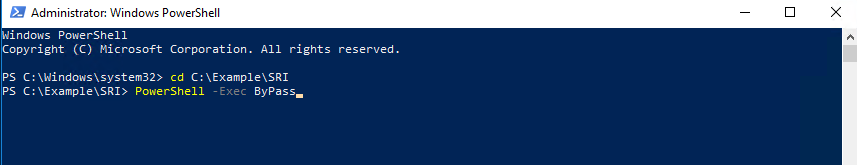
\includegraphics[width=1\linewidth]{assets/ps_bypass.png}
    \caption{PowerShell Bypass}
\end{figure} \ \\
Now you can run the SRI by open the sri.ps1 file. You find more details to the different modes in the section below.
\begin{figure}[H]
    \centering
    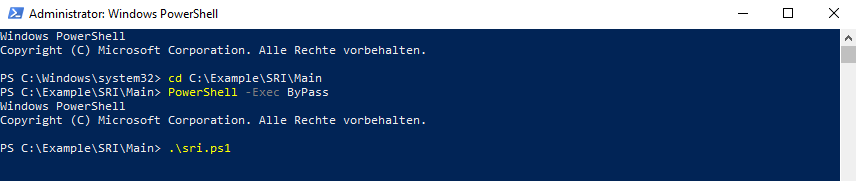
\includegraphics[width=1\linewidth]{assets/sri_ps1.png}
    \caption{PowerShell Bypass}
\end{figure} \ \\

\subsection{SRI modes}
As described in \nameref{GeneralInfo} there are four different modes to run the SRI. These modes are described more precisely in this chapter. These are the four modes:
\begin{itemize}
    \item \textbf{\textit{-Online, -Offline, -GroupPolicy and -AllGroupPolicies}}
\end{itemize}
\begin{lstlisting}[caption=]
PS C:\>./sri.ps1 [-Online] [-OnlineExportPath <String>] [-CAPI2LogSize <Int32>]

PS C:\>./sri.ps1 [-Offline] [[-AuditPolicies]] [[-EventLogs]] [-ImportPath] <String> 
                       [[-ExportPath] <String>] [-CAPI2LogSize <Int32>]

PS C:\>./sri.ps1 [-GroupPolicy] [-GroupPolicyName] <String>

PS C:\>./sri.ps1 [-AllGroupPolicies]
\end{lstlisting}
\clearpage \ \\
The parameters ''-OnlineExportPath'', ''-ImportPath'' and ''-ExportPath'' are Strings, for example:\ \\
\begin{lstlisting}[caption=]
    C:\Example\Path
\end{lstlisting} \ \\
The parameters ''-CAPI2LogSize''is a Integer, for example:\ \\
\begin{lstlisting}[caption=]
    4000000
\end{lstlisting}
The parameters ''-GroupPolicyName''is a String, for example:\ \\
\begin{lstlisting}[caption=]
    Default Group Policy
\end{lstlisting}

\vspace{0.5cm}
\textsc{\textbf{Note:}}\textit{ Mandatory parameter are \underline{underlined}.}
\vspace{0.5cm}
\begin{tcolorbox}
    \paragraph{\underline{-Online}} \ \\\\
    The current system which is calling the script will be checked on its readiness.
    \vspace{0.3cm}
    \begin{center}
        \textsc{Parameter}
    \end{center}
    \vspace{-0.5cm}
    \begin{table}[H]
        \def\arraystretch{2}
        \centering
        \begin{tabular}{ p{4cm}  p{10cm} }  \hline
            \textbf{No parameter} & The result PDF will be saved to the current path \\ \hline
            \textbf{-OnlineExportPath} & The result PDF will be saved to this path \\ \hline
            \textbf{-CAPI2LogSize} & Definition of the CAPI2 log size suitable for the environment. By default this value is set to 4MB as recommended from Microsoft  \\ \hline
        \end{tabular}
    \end{table}
\end{tcolorbox}

\begin{tcolorbox}
    \paragraph{\underline{-Offline}} \ \\\\ Some system will be checked on its readiness - by default audit policies and event log are analysed. Export files of this system are required.
    \vspace{0.3cm}
    \begin{center}
        \textsc{Parameter}
    \end{center}
    \vspace{-0.5cm}
    \begin{table}[H]
        \def\arraystretch{2}
        \centering
        \begin{tabular}{ p{4cm}  p{10cm} }  \hline
            \textbf{\underline{-ImportPath}} & Defines where the required files rsop.xml\footnote{XML-Export of Resultant Set of Policy}, windowslogs.csv\footnote{Export of }, appandservlogs.csv\footnote{Export of } remain for analysis. \\ 
            & The result PDF will be saved to the current path \\ \hline
            \textbf{-AuditPolicies} & Checks only the audit policies. \\
            & The result PDF will be saved to the current path \\ 
            & \textbf{\underline{-ImportPath}} requires rsop.xml \\\hline
            \textbf{-EventLogs} & Checks only the event logs \\
            & The result PDF will be saved to the current path \\ 
            & \textbf{\underline{-ImportPath}} requires windowslogs.csv and appandservlogs.csv\\\hline
            \textbf{-ExportPath} & The result PDF will be saved to this path \\ \hline
            \textbf{-CAPI2LogSize} & Definition of the CAPI2 log size suitable for the environment. By default this value is set to 4MB as recommended from Microsoft  \\ \hline
        \end{tabular}
    \end{table}
\end{tcolorbox}

\begin{tcolorbox}
    \paragraph{\underline{-GroupPolicy}} \ \\\\ Audit policies from a specific group policy are analysed.
    \vspace{0.3cm}
    \begin{center}
        \textsc{Parameter}
    \end{center}
    \vspace{-0.5cm}
    \begin{table}[H]
        \def\arraystretch{2}
        \centering
        \begin{tabular}{ p{4cm}  p{10cm} } \hline
            \textbf{\underline{-GroupPolicyName}} & The name of the group policy to be analysed \\ \hline
        \end{tabular}
    \end{table}
\end{tcolorbox}

\begin{tcolorbox}
    \paragraph{\underline{-AllGroupPolicies}} \ \\\\
    All audit policies from every group policy in the current domain are analysed.\\
    The result PDF will be saved to the current path
\end{tcolorbox}


\end{document}